\newpage
\graphicspath{{../timhieucungbi/hoclamthamtu/}}
\begingroup
\AddToShipoutPicture*{\put(92,608){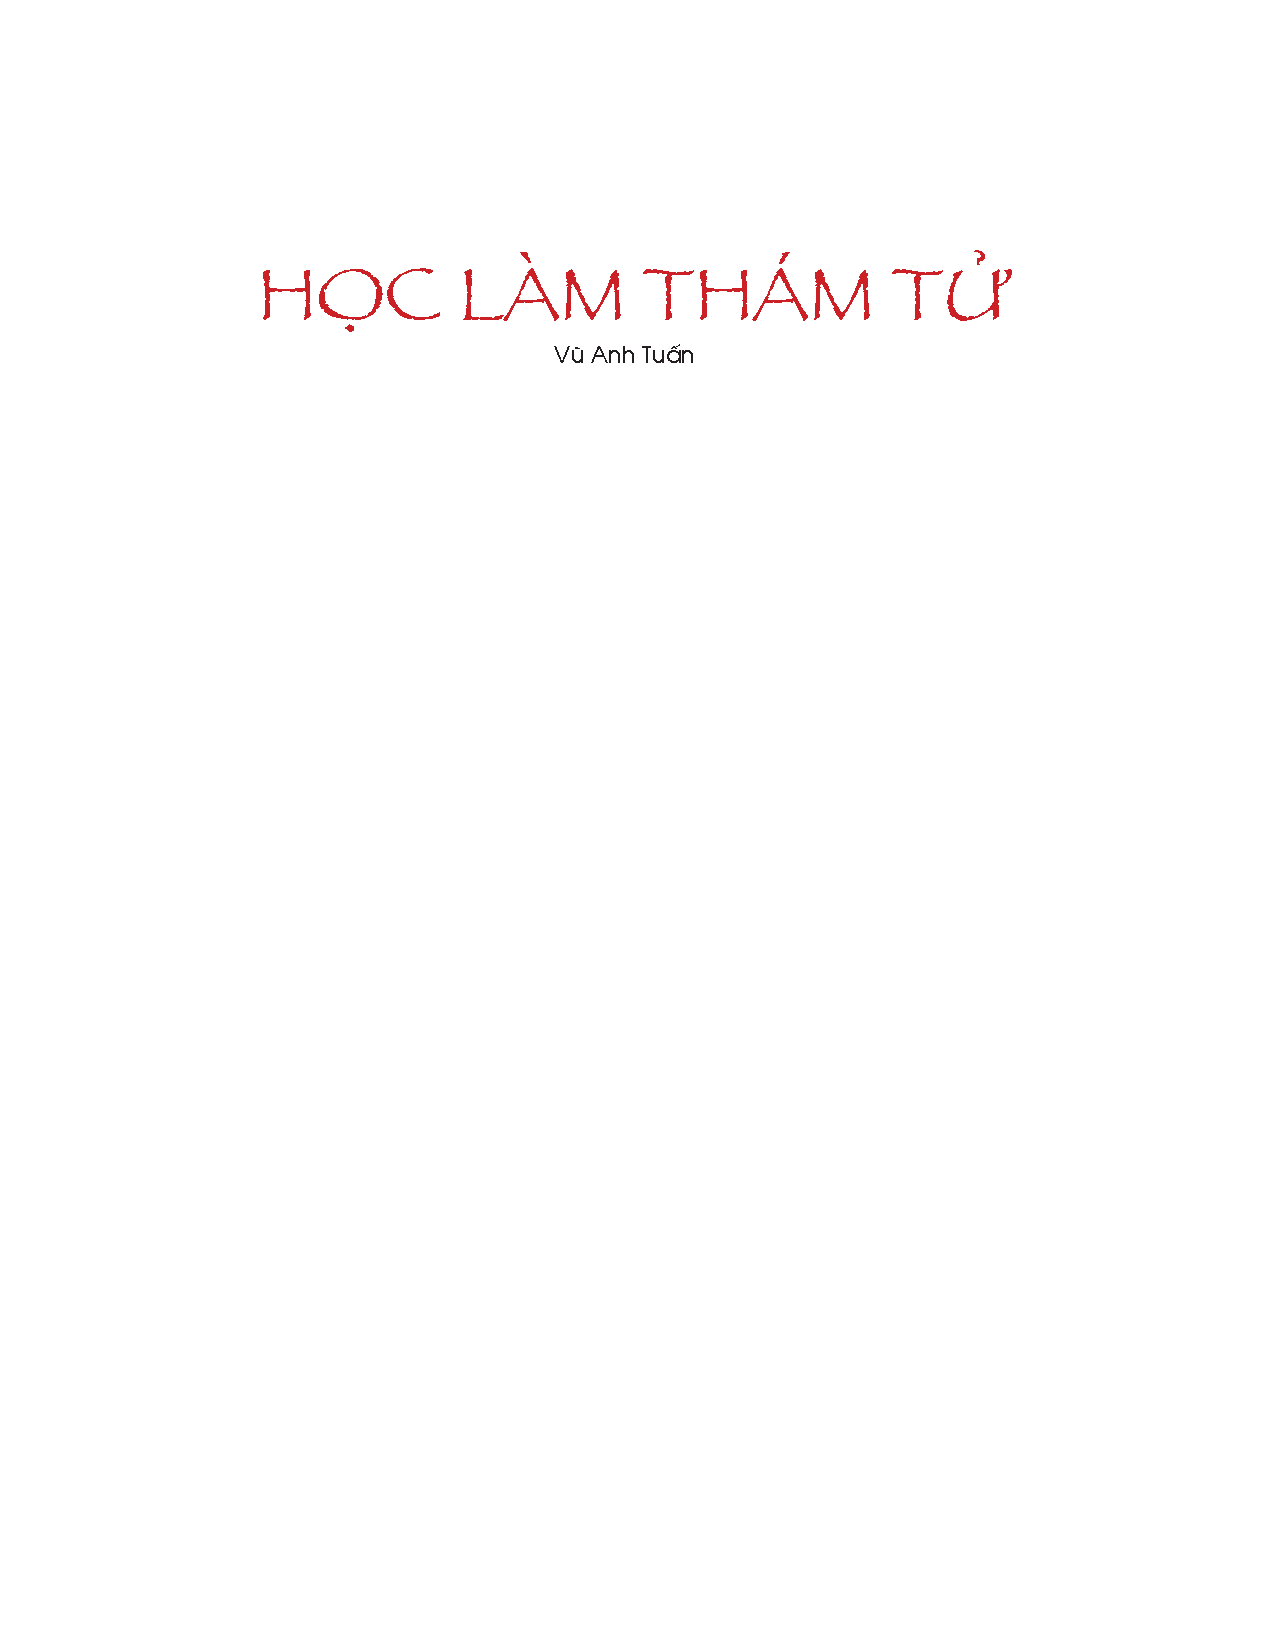
\includegraphics[scale=0.85]{tieude.pdf}}} % %Image background
\centering
\endgroup
\vspace*{25pt}
	Khi Bi bắt đầu học làm thám tử, việc đầu tiên Bi phải học là cách xác định phương hướng. Người thầy đầu tiên của Bi là Ông ngoại. Ông chỉ cho Bi cách xác định hướng Đông, Tây, Nam, Bắc như sau:
	\vskip 0.1cm
	\textit{“Mặt trời mọc ở hướng Đông, lặn ở hướng Tây, và mặt trời mọc và lặn ở hai hướng đối diện nhau. Vì thế, cháu có thể căn cứ vào hướng mặt trời mọc, hay hướng mặt trời lặn để xác định các hướng của đất trời. Cụ thể là thế này:}
	\vskip 0.1cm
	\begin{wrapfigure}{r}{0.34\textwidth}
		\centering
		\vspace*{-15pt}
		\captionsetup{labelformat= empty, justification=centering}
		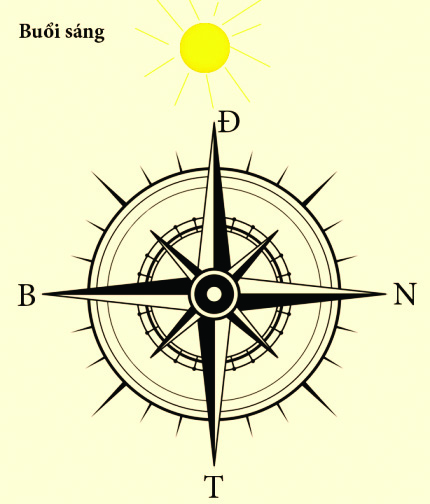
\includegraphics[width=0.3\textwidth]{pic1}
		\caption{\small\textit{Hình $1$: Xác định hướng theo hướng mặt trời mọc}}
		\vspace*{-10pt}
	\end{wrapfigure}
	\textit{Buổi sáng, khi thức dậy, nếu cháu đứng dang hai tay ngang vai và nhìn về phía mặt trời, thì trước mặt cháu là hướng Đông (viết tắt là \textnormal{Đ}), sau lưng cháu là hướng Tây (viết tắt là \textnormal{T}), tay phải của cháu chỉ về hướng Nam (viết tắt là \textnormal{N}), và tay trái của cháu chỉ về hướng Bắc (viết tắt là \textnormal{B}).”} (Xem Hình $1$.)
	\vskip 0.1cm
	\textbf{\color{toancuabi}Ví dụ $\pmb1.$} Trên mặt đất vẽ hình vuông $ABCD$. Biết rằng, đỉnh $D$ của hình vuông nằm ở hướng mặt trời lặn. Hỏi các đỉnh $A, B, C$ nằm ở  hướng nào?
	\vskip 0.1cm
	\begin{wrapfigure}{l}{0.35\textwidth}
		\centering
%		\vspace*{-5pt}
		\captionsetup{labelformat= empty, justification=centering}
		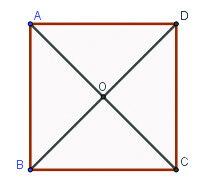
\includegraphics[width=0.38\textwidth]{pic2}
		\caption{\small\textit{Hình $2.$}}
		\vspace*{-15pt}
	\end{wrapfigure}
	\textbf{\color{toancuabi}Cùng Bi suy luận:}
	\vskip 0.1cm
	-- Để dễ dàng quan sát cả bốn điểm $A, B, C, D$, ta nên đứng ở tâm $O$ của hình vuông $ABCD$ (xem Hình $2$);
	\vskip 0.1cm
	-- Vì đề bài cho điểm $D$ nằm ở hướng mặt trời lặn; mà mặt trời lặn ở hướng Tây, nên điểm $D$ nằm ở hướng Tây. Đối diện với hướng Tây là hướng Đông, nên đỉnh $B$ nằm ở hướng Đông;
	\vskip 0.1cm
	-- Bây giờ, ta sẽ quay mặt về phía điểm $B$, tức là, quay mặt về hướng Đông, và dang hai tay ngang vai. Khi đó, tay phải của ta sẽ chỉ về phía điểm $A$, và tay trái chỉ về phía điểm $C$. Vì thế, theo lời dạy của ông nội Bi, điểm $A$ nằm ở hướng Nam, và điểm $C$ nằm ở hướng Bắc.
	\vskip 0.1cm
	\textbf{\color{toancuabi}Ví dụ $\pmb2.$} Bốn góc vườn trồng cây cảnh của ông ngoại Bi nằm ở bốn hướng Đông, Tây, Nam, Bắc (mỗi góc nằm ở một hướng). Ở bốn góc vườn, ông trồng bốn khóm hoa, gồm cúc, huệ, hồng, dơn; mỗi khóm hoa được trồng ở một góc vườn và ở mỗi góc vườn chỉ trồng một khóm hoa. Biết rằng, hai góc vườn phía Tây và phía Bắc không trồng huệ. Nếu đi một vòng quanh vườn, theo chiều quay của kim đồng hồ, thì sẽ thấy khóm huệ được trồng giữa khóm cúc và góc vườn phía Nam, còn khóm dơn thì được trồng giữa khóm hồng và góc vườn phía Bắc. Đố em biết, ở mỗi góc vườn, ông ngoại Bi đã trồng hoa gì?
	\vskip 0.1cm
	\textbf{\color{toancuabi}Cùng Bi suy luận:}
	\vskip 0.1cm
	-- Vì liên quan đến vườn cây cảnh của ông ngoại Bi có khá nhiều thông tin, và xem ra cũng có phần “phức tạp”, nên sẽ chẳng dễ chịu chút nào khi chúng mình cố gắng hình dung ra cái vườn ấy ở trong đầu để suy luận; phải không các em? Thế nên, chúng mình sẽ tìm cách thể hiện cái vườn ấy, cùng các thông tin liên quan đến nó, bằng hình ảnh, để khắc phục cái “chẳng dễ chịu chút nào” nói trên nhé.
	\vskip 0.1cm
	\begin{wrapfigure}{r}[0pt]{0.59\linewidth}
		\vspace*{-20pt}
		\centering
		\captionsetup{labelformat=empty, justification=centering}
		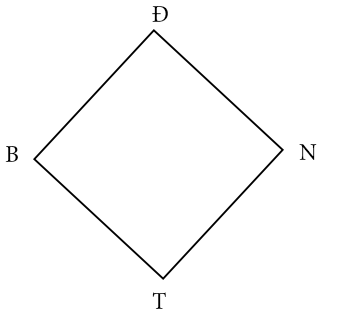
\includegraphics[width= 0.29\textwidth]{pic3}
		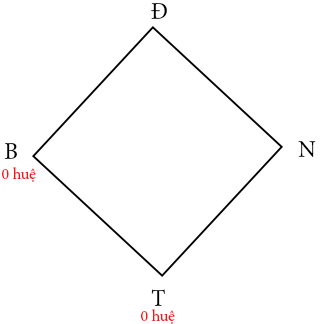
\includegraphics[width=0.29\textwidth]{pic4}
		\caption{\small\textit{Hình $3.$ \hspace*{50pt}Hình $4.$}}
		\vspace*{-15pt}
	\end{wrapfigure}
	-- Trước hết, chúng mình sẽ thể hiện cái vườn của ông ngoại Bi bằng một hình vuông, và tại mỗi đỉnh của nó có ghi tên hướng của góc vườn tại đỉnh ấy (xem Hình $3$).
	\vskip 0.15cm
	-- Tiếp theo, vì “hai góc vườn phía Tây và phía Bắc không trồng huệ” nên chúng mình sẽ ghi “0 huệ” vào hai đỉnh T (Tây) và B (Bắc) (xem Hình $4$).
	\vskip 0.15cm
	-- Bây giờ, đến lượt giả thiết “Nếu đi một vòng quanh vườn, theo chiều quay của kim đồng hồ, thì sẽ thấy khóm huệ được trồng giữa khóm cúc và góc vườn phía Nam, còn khóm dơn thì được trồng giữa khóm hồng và góc vườn phía Bắc”. Chúng mình sẽ thể hiện việc đi vòng quanh vườn (cho đỡ phải hình dung trong đầu) bằng các mũi tên cong, như ở Hình $5$.
	\vskip 0.1cm
	\begin{wrapfigure}{r}[0pt]{0.35\linewidth}
		\vspace*{-15pt}
		\centering
		\captionsetup{labelformat=empty, justification=centering}
		\hspace*{-10pt}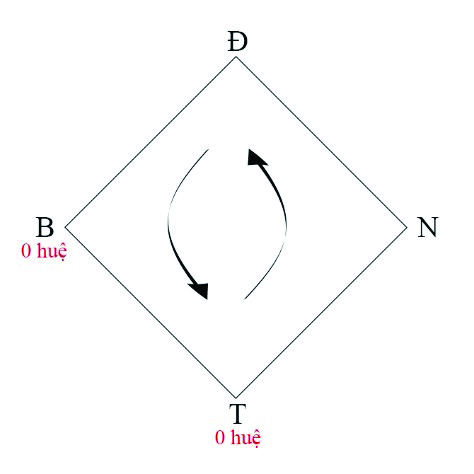
\includegraphics[width= 0.29\textwidth]{pic5}
		\caption{\textit{\small Hình $5.$}}
		\vspace*{5pt}
		\hspace*{-10pt}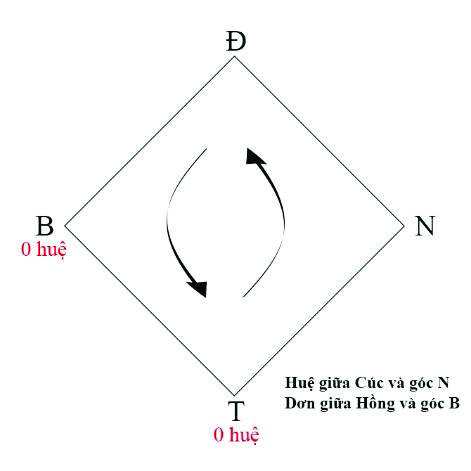
\includegraphics[width=0.29\textwidth]{pic6}
		\caption{\small\textit{Hình $6.$}}
		\vspace*{-20pt}
	\end{wrapfigure}
	\vskip 0.15cm
	Tiếp theo, chúng mình ghi phần còn lại của giả thiết nêu trên một cách vắn tắt bên cạnh hình vuông ở Hình $5$, như ở Hình $6$.
	\vskip 0.15cm
	-- Thế là, tới lúc này, chúng mình đã thể hiện được toàn bộ các giả thiết của bài toán ở Ví dụ $2$ bằng Hình $6$. Công việc bây giờ, hiển nhiên là quan sát Hình $6$ và suy luận, để tìm ra câu trả lời cho câu hỏi của bài toán đã ra.
	\vskip 0.15cm
	-- Chắc hẳn các em cũng đồng ý rằng, để kết nối các thông tin ở Hình $6$ (tức, các giả thiết của bài toán đã ra), nhằm tìm ra con đường đi tới câu trả lời cho câu hỏi của bài toán, trước hết, chúng mình cần làm rõ (để hiểu rõ) thông tin “huệ ở giữa cúc và góc Nam (cũng như, dơn ở giữa hồng và góc Bắc), nếu đi theo chiều kim đồng hồ”.
	\vskip 0.15cm
	Các em ạ, trong Toán học, cũng như trong sinh hoạt đời sống, với $A, B, C$ là ba vị trí (hay, ba điểm) không cùng nằm trên một đường thẳng (còn nói gọn là “\textit{không thẳng hàng}”):
	\vskip 0.15cm
	+ Khi nói, \textit{“vị trí $A$ (\textnormal{hay}, điểm $A$) nằm giữa (\textnormal{hay}, ở giữa) hai vị trí (\textnormal{hay}, hai điểm) \textbf{\color{toancuabi}$\pmb B$ và $\pmb C$}, nếu đi theo chiều kim đồng hồ (\textnormal{hay}, xét theo chiều kim đồng hồ)” (\textnormal{hoặc còn} nói một cách khác, “ba vị trí (\textnormal{hay}, ba điểm) $B, A, C$ nằm theo thứ tự đó, xét theo chiều kim đồng hồ”) thì \textbf{\color{toancuabi}hiểu là}: khi đi trên một cung tròn, từ vị trí (\textnormal{hay}, điểm) $B$ đến vị trí (\textnormal{hay}, điểm) $C$, theo chiều kim đồng hồ, thế nào ta cũng gặp (\textnormal{hay}, đi qua) vị trí (\textnormal{hay}, điểm) $A$ trên đường đi} (xem hình minh họa dưới đây -- Hình $7$).
%	\begin{figure}[H]
%		\centering
%		\vspace*{-15pt}
%		\captionsetup{labelformat= empty, justification=centering}
%		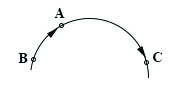
\includegraphics[width=0.35\textwidth]{pic7}
%		\caption{\small\textit{Hình 7}}
%		\vspace*{-15pt}
%	\end{figure}
\vskip 0.1cm
		\begin{wrapfigure}{l}[0pt]{0.35\linewidth}
		\vspace*{-15pt}
		\centering
		\captionsetup{labelformat=empty, justification=centering}
		\hspace*{-10pt}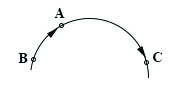
\includegraphics[width= 0.35\textwidth]{pic7}
		\caption{\textit{\small Hình $7.$}}
		
		\vspace*{10pt}
		\hspace*{-10pt}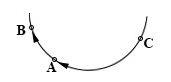
\includegraphics[width=0.35\textwidth]{pic8}
		\caption{\small\textit{Hình $8.$}}
		
		\vspace*{10pt}
		\captionsetup{labelformat=empty, justification=centering}
		\hspace*{-10pt}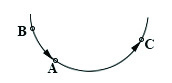
\includegraphics[width= 0.35\textwidth]{pic9}
		\caption{\textit{\small Hình $9.$}}
		
		\vspace*{-20pt}
	\end{wrapfigure}
	+ Còn khi nói, “\textit{vị trí $A$ (\textnormal{hay}, điểm $A$) nằm giữa (\textnormal{hay}, ở giữa) hai vị trí (\textnormal{hay}, hai điểm) \textbf{\color{toancuabi}$\pmb C$ và $\pmb B$}, nếu đi theo chiều kim đồng hồ (\textnormal{hay}, xét theo chiều kim đồng hồ)” (\textnormal{hoặc còn} nói một cách khác, “ba vị trí (\textnormal{hay}, ba điểm) $C, A, B$ nằm theo thứ tự đó, xét theo chiều kim đồng hồ”) thì \textbf{\color{toancuabi}hiểu là}: khi đi trên một cung tròn, từ vị trí (\textnormal{hay}, điểm) $C$ đến vị trí (\textnormal{hay}, điểm) $B$, theo chiều kim đồng hồ, thế nào ta cũng gặp (\textnormal{hay}, đi qua) vị trí (\textnormal{hay}, điểm) $A$ trên đường đi} (xem hình minh họa dưới đây -- Hình $8.$).
%	\begin{figure}[H]
%		\centering
%		\vspace*{-15pt}
%		\captionsetup{labelformat= empty, justification=centering}
%		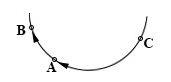
\includegraphics[width=0.35\textwidth]{pic8}
%		\caption{\small\textit{Hình 8}}
%		\vspace*{-15pt}
%	\end{figure}
	\vskip 0.1cm
	+ Khi nói, “\textit{vị trí $A$ (\textnormal{hay}, điểm $A$) nằm giữa (\textnormal{hay}, ở giữa) hai vị trí (\textnormal{hay}, hai điểm) \textbf{\color{toancuabi}$\pmb B$ và $\pmb C$}, nếu đi theo chiều ngược chiều kim đồng hồ (\textnormal{hay}, xét theo chiều ngược chiều kim đồng hồ)” (\textnormal{hay còn} nói một cách khác, “ba vị trí (\textnormal{hay}, ba điểm) $B, A, C$ nằm theo thứ tự đó, xét theo chiều ngược chiều kim đồng hồ”) thì \textbf{\color{toancuabi}hiểu là}: khi đi trên một cung tròn, từ vị trí (\textnormal{hay}, điểm) $B$ đến vị trí (\textnormal{hay}, điểm) $C$, theo chiều ngược chiều kim đồng hồ, thế nào ta cũng gặp (\textnormal{hay}, đi qua) vị trí (\textnormal{hay}, điểm) $A$ trên đường đi} (xem hình minh họa dưới đây -- Hình $9.$).
	\vskip 0.1cm
%	\begin{figure}[H]
%		\centering
%		\vspace*{-15pt}
%		\captionsetup{labelformat= empty, justification=centering}
%		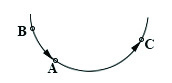
\includegraphics[width=0.35\textwidth]{pic9}
%		\caption{\small\textit{Hình 9}}
%		\vspace*{-5pt}
%	\end{figure}
	+ Cuối cùng, khi nói, “\textit{vị trí $A$ (\textnormal{hay}, điểm $A$) nằm giữa (\textnormal{hay}, ở giữa) hai vị trí (\textnormal{hay}, hai điểm) \textbf{\color{toancuabi}$\pmb C$ và $\pmb B$}, nếu đi theo chiều ngược chiều kim đồng hồ (\textnormal{hay}, xét theo chiều ngược chiều kim đồng hồ)” (\textnormal{hay còn} nói một cách khác, “ba vị trí (\textnormal{hay}, ba điểm) $C, A, B$ nằm theo thứ tự đó, xét theo chiều ngược chiều kim đồng hồ”) thì \textbf{\color{toancuabi}hiểu là}: khi đi trên một cung tròn, từ vị trí (\textnormal{hay}, điểm) $C$ đến vị trí (\textnormal{hay}, điểm) $B$, theo chiều ngược chiều kim đồng hồ, thế nào ta cũng gặp (\textnormal{hay}, đi qua) vị trí (\textnormal{hay}, điểm) $A$ trên đường đi} (xem hình minh họa dưới đây -- Hình $10$).
	\vskip 0.1cm
	\begin{wrapfigure}{l}[0pt]{0.35\linewidth}
		\centering
		\vspace*{-10pt}
		\captionsetup{labelformat= empty, justification=centering}
		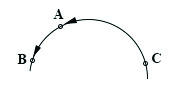
\includegraphics[width=0.35\textwidth]{pic10}
		\caption{\small\textit{Hình $10.$}}
		\vspace*{-10pt}
	\end{wrapfigure}
	-- Sau khi đã hiểu rõ quan hệ “ở giữa” như trên, hiển nhiên chúng mình thấy rằng, “huệ ở giữa cúc và góc N, nếu đi theo chiều kim đồng hồ” có nghĩa là “khi đi từ góc có trồng cúc đến góc N, theo chiều kim đồng hồ, thế nào ta cũng đi qua góc có trồng huệ”. 
	\vskip 0.1cm
	\begin{wrapfigure}{r}[0pt]{0.35\linewidth}
		\vspace*{-25pt}
		\centering
		\captionsetup{labelformat=empty, justification=centering}
		\hspace*{-7pt}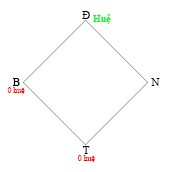
\includegraphics[width= 0.29\textwidth]{pic11}
		
		\vspace*{-5pt}
		\caption{\textit{\small Hình $11.$}}
		\hspace*{-7pt}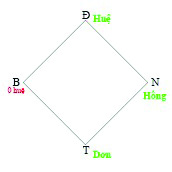
\includegraphics[width= 0.29\textwidth]{pic12}
		
		\vspace*{-10pt}
		\caption{\textit{\small Hình $12.$}}
		\vspace*{-25pt}
		
		\hspace*{-7pt}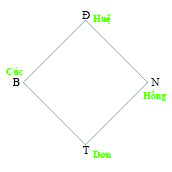
\includegraphics[width= 0.29\textwidth]{pic13}
		
		\vspace*{-15pt}
		\caption{\textit{\small Hình $13.$}}
		\vspace*{-25pt}
	\end{wrapfigure}
	\vskip 0.1cm
	Từ đây, quan sát Hình $6$, rõ ràng suy ra, cúc không thể được trồng ở góc Đ (vì khi đó, đi theo chiều kim đồng hồ từ góc Đ đến góc N, ta không đi qua góc nào cả). Như thế, cúc chỉ có thể được trồng ở góc T hoặc góc B; suy ra, huệ chỉ có thể được trồng ở góc B hoặc góc Đ. Mà ở góc B “0 huệ” nên huệ phải được trồng ở góc Đ (xem Hình $11$).
	\vskip 0.1cm
	-- Tương tự trên, từ “dơn ở giữa hồng và góc B, nếu đi theo chiều kim đồng hồ”, quan sát Hình $6$, chúng mình suy ra hồng chỉ có thể được trồng ở góc Đ hoặc góc N. Mà ở góc Đ đã trồng huệ, nên hồng phải được trồng ở góc N, và do đó, dơn phải được trồng ở góc T (xem Hình $12$).
	\vskip 0.1cm
%	\begin{wrapfigure}{r}[0pt]{0.55\linewidth}
%			\vspace*{-20pt}
%			\centering
%			\captionsetup{labelformat=empty, justification=centering}
%			\hspace*{-7pt}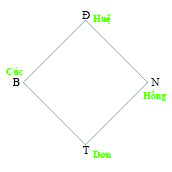
\includegraphics[width= 0.29\textwidth]{pic13}
%			
%			\vspace*{-15pt}
%			\caption{\textit{\small Hình 13}}
%			\vspace*{-20pt}
%		\end{wrapfigure}
	-- Vì chỉ còn cúc và góc B nên cúc phải được trồng ở đó rồi, các em nhỉ? (xem Hình $13$)
	\vskip 0.1cm
	Sau khi Bi đã  thành thạo bốn hướng chính là Đông, Tây, Nam, Bắc, ông ngoại dạy thêm cho Bi các hướng phụ, là hướng Đông Bắc (viết tắt là ĐB), Đông Nam (viết tắt là ĐN), Tây Bắc (viết tắt là TB) và Tây Nam (viết tắt là TN). Ông bảo:
	\vskip 0.1cm
	“\textit{Cháu ạ, hướng Đông Bắc là hướng nằm ở chính giữa hướng Đông và hướng Bắc; hướng Đông Nam là hướng nằm ở chính giữa hướng Đông và hướng Nam; hướng Tây Bắc là hướng nằm ở chính giữa hướng Tây và hướng Bắc; và cuối cùng, hướng Tây Nam là hướng nằm ở chính giữa hướng Tây và hướng Nam}.” (xem Hình $14$).
	\begin{figure}[H]
		\centering
%		\vspace*{-5pt}
		\captionsetup{labelformat= empty, justification=centering}
		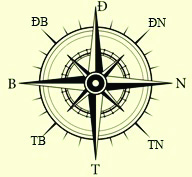
\includegraphics[width=0.38\textwidth]{pic14}
		\caption{\small\textit{Hình $14.$}}
		\vspace*{-10pt}
	\end{figure}
	Ông ngoại lại còn dạy cho Bi biết, có những lúc, nhà thám tử không xác định hướng theo Đông, Tây, Nam, Bắc, mà xác định bằng hướng chỉ của kim giờ trên mặt đồng hồ. Người ta gọi những hướng được xác định theo cách như thế là \textit{hướng “giờ”}. Ông dạy Bi:
	\vskip 0.1cm
	“\textit{Mỗi vị trí của kim giờ trên mặt đồng hồ (cơ) xác định một hướng, và người ta dùng thời gian mà kim giờ chỉ (khi nằm ở vị trí ấy) làm tên gọi cho hướng mà nó xác định. Ví dụ, vị trí của kim giờ lúc nó chỉ $12$ giờ xác định hướng $12$ giờ (xem Hình $15$); vị trí của kim giờ lúc nó chỉ $4$ giờ $30$ phút xác định hướng $4$ giờ $30$ phút (xem Hình $16$); ...; hay như, hướng $6$ giờ là hướng xác định bởi vị trí của kim giờ lúc nó chỉ $6$ giờ (xem Hình $17$), hướng $1$ giờ $30$ phút là hướng xác định bởi vị trí của kim giờ vào lúc $1$ giờ $30$ phút (xem Hình $18$), ... Một điều cực kỳ quan trọng cháu phải nhớ: \textbf{\color{toancuabi}Khi xác định hướng theo cách này}, mặt đồng hồ phải được đặt nằm vuông góc với thân người, sao cho số $12$ trên mặt đồng hồ nằm ở hướng nhìn thẳng của mắt người đang xác định hướng; nghĩa là, \textbf{\color{toancuabi}hướng $12$ giờ phải là hướng mắt nhìn thẳng của người định hướng}}.”
		\begin{figure}[H]
		\centering
		\vspace*{4pt}
		\captionsetup{labelformat= empty, justification=centering}
		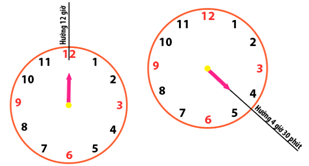
\includegraphics[width=0.465\textwidth]{pic15}
		%\caption{\small\textit{Hình 15 \hspace*{70pt Hình 16}}}
		%\vspace*{5pt}
		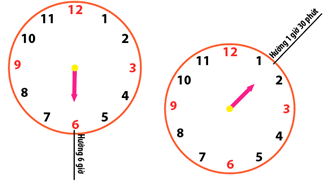
\includegraphics[width=0.465\textwidth]{pic16}
		\caption{\small\textit{Hình $17$ \hspace*{70pt} Hình $18$}}
		\vspace*{-10pt}
	\end{figure}
	\textbf{\color{toancuabi}Câu đố.} Đố em biết:
	\vskip 0.05cm
	-- Kim giờ trong Hình $19$ xác định hướng  mấy giờ?
	\vskip 0.05cm
	-- Kim giờ trong Hình $20$ xác định hướng  mấy giờ?
		\begin{figure}[H]
		\centering
		\vspace*{-5pt}
		\captionsetup{labelformat= empty, justification=centering}
		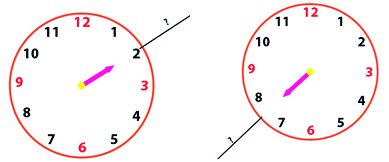
\includegraphics[width=0.465\textwidth]{pic17}
		\caption{\small\textit{Hình $19.$ \hspace*{80pt} Hình $20.$}}
		\vspace*{-10pt}
	\end{figure}
	\textbf{\color{toancuabi}Ví dụ $\pmb3.$} Trong Hình $21$, người quan sát đứng quay mặt về hướng Đông; còn ở Hình $22$, người quan sát đứng quay mặt về hướng Nam. Em hãy cho biết:
			\begin{figure}[H]
		\centering
		\vspace*{-5pt}
		\captionsetup{labelformat= empty, justification=centering}
		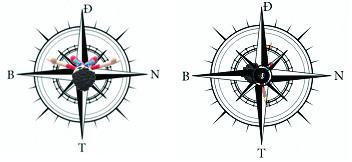
\includegraphics[width=0.48\textwidth]{pic18}
		\caption{\small\textit{Hình $21$ \hspace*{80pt} Hình 22}}
		\vspace*{-5pt}
	\end{figure}
	-- Ở Hình $21$, hướng $9$ giờ là hướng nào trong hệ Đ -- T -- N -- B?
	\vskip 0.05cm
	-- Ở Hình $22$, hướng $10$ giờ $30$ phút là hướng nào trong hệ Đ -- T -- N -- B?
	\vskip 0.05cm
	\textbf{\color{toancuabi}Cùng Bi suy luận:}
	\vskip 0.1cm
	-- Thông thường, để xác định hướng “giờ”, người ta phải tưởng tượng trong đầu chiếc mặt đồng hồ, có một chiếc kim chỉ giờ ở đó. Nhưng chúng mình bây giờ mới đang tập, lại sẵn có hình, nên để tránh phải tưởng tượng nhiều, chúng mình sẽ ghi viền quanh la bàn các con số trên mặt đồng hồ, và coi luôn mặt la bàn là mặt đồng hồ; còn chiếc kim giờ thì phải tưởng tượng trong đầu thôi, vì vẽ ra thì rối hình lắm.
	\vskip 0.1cm
	-- Theo điều “cực kỳ quan trọng” mà ông ngoại Bi dạy, vì ở Hình $21$, người quan sát đứng quay mặt về hướng Đ, nên chúng mình phải ghi số $12$ vào chỗ chữ Đ; còn ở Hình $22$, người quan sát đứng quay mặt về hướng N, nên chúng mình phải ghi số $12$ vào chỗ chữ N. Sau đó, chúng mình lần lượt ghi tiếp, theo chiều kim đồng hồ, các số từ $1$ đến $11$, sao cho các số được ghi nằm cách đều nhau (xem Hình $23$ và Hình $24$).
	\begin{figure}[H]
		\centering
		\vspace*{-5pt}
		\captionsetup{labelformat= empty, justification=centering}
		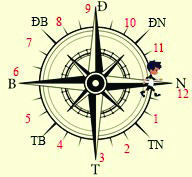
\includegraphics[width=0.48\textwidth]{pic19}
		\caption{\small\textit{Hình $23.$ \hspace*{80pt} Hình $24.$}}
		\vspace*{-15pt}
	\end{figure}
	-- Vì hướng $9$ giờ được xác định bởi vị trí của kim giờ, khi nó chỉ $9$ giờ; mà lúc $9$ giờ, kim giờ chỉ vào số $9$ nên suy ra, ở Hình $23$, hướng $9$ giờ là hướng Bắc (B). Tương tự như thế, vì lúc $10$ giờ $30$ phút, kim giờ chỉ vào điểm chính giữa số $10$ và số $11$, xét theo chiều kim đồng hồ, nên ở Hình $24$, hướng $10$ giờ $30$ phút là hướng Đông Nam (ĐN).
	\vskip 0.1cm
	Bi còn phải hoàn thành một số thử thách nữa của ông ngoại về xác định hướng, mới có thể nhập môn Thám tử được. Em hãy cùng Bi làm các bài tập dưới đây nhé.
	\vskip 0.1cm
	\textbf{\color{toancuabi}Bài tập $\pmb1.$} Trong một buổi chiều tà, không mưa, Pi đứng quay lưng về phía mặt trời, hai tay dang ngang vai. Hỏi tay trái của Pi chỉ về hướng nào trong hệ Đ -- T -- N -- B? Tay phải của Pi chỉ về hướng nào trong hệ Đ -- T -- N -- B?
	\vskip 0.1cm
	\textbf{\color{toancuabi}Bài tập $\pmb2.$} Hình $25$ là bản đồ khu vực Hồ Gươm và một số địa danh quanh Hồ Gươm. Giả sử Em đang đứng ở Đền Ngọc Sơn, và quay lưng về phía Tháp Rùa. Em hãy cho biết:
	\begin{figure}[H]
		\centering
		\vspace*{-5pt}
		\captionsetup{labelformat= empty, justification=centering}
		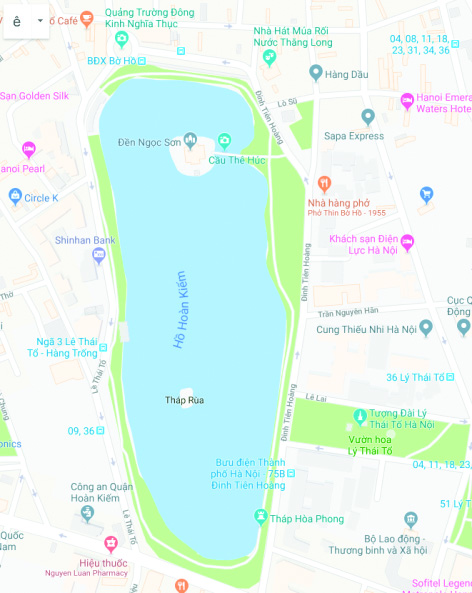
\includegraphics[width=0.3\textwidth]{pic25}
		\caption{\small\textit{Hình $25$}}
		\vspace*{-5pt}
	\end{figure}
	$a)$ Địa danh nào nằm ở hướng $11$ giờ và địa danh nào nằm ở hướng $1$ giờ?
	\vskip 0.1cm
	$b)$ Tháp Rùa nằm ở hướng mấy giờ?